\documentclass{beamer}
\usepackage{amsmath}
\usepackage[english]{babel} %set language; note: after changing this, you need to delete all auxiliary files to recompile
\usepackage[utf8]{inputenc} %define file encoding; latin1 is the other often used option
\usepackage{csquotes} % provides context sensitive quotation facilities
\usepackage{graphicx} %allows for inserting figures
\usepackage{booktabs} % for table formatting without vertical lines
\usepackage{textcomp} % allow for example using the Euro sign with \texteuro
\usepackage{stackengine}
\usepackage{wasysym}
\usepackage{tikzsymbols}
\usepackage{textcomp}
% ELIMINAR COMANDOS DE NAVEGACION%%%%%%%%%%%
\setbeamertemplate{navigation symbols}

%\newcommand{\bubblethis}[2]{
 %       \tikz[remember picture,baseline]{\node[anchor=base,inner sep=0,outer sep=0]%
 %       (#1) {\underline{#1}};\node[overlay,cloud callout,callout relative pointer={(0.2cm,-0.7cm)},%
 %       aspect=2.5,fill=yellow!90] at ($(#1.north)+(-0.5cm,1.6cm)$) {#2};}%
 %   }%
%\tikzset{face/.style={shape=circle,minimum size=4ex,shading=radial,outer sep=0pt,
 %       inner color=white!50!yellow,outer color= yellow!70!orange}}

%% Some commands to make the code easier
\newcommand{\emoticon}[1][]{%
  \node[face,#1] (emoticon) {};
  %% The eyes are fixed.
  \draw[fill=white] (-1ex,0ex) ..controls (-0.5ex,0.2ex)and(0.5ex,0.2ex)..
        (1ex,0.0ex) ..controls ( 1.5ex,1.5ex)and( 0.2ex,1.7ex)..
        (0ex,0.4ex) ..controls (-0.2ex,1.7ex)and(-1.5ex,1.5ex)..
        (-1ex,0ex)--cycle;}
\newcommand{\pupils}{
  %% standard pupils
  \fill[shift={(0.5ex,0.5ex)},rotate=80] 
       (0,0) ellipse (0.3ex and 0.15ex);
  \fill[shift={(-0.5ex,0.5ex)},rotate=100] 
       (0,0) ellipse (0.3ex and 0.15ex);}

\newcommand{\emoticonname}[1]{
  \node[below=1ex of emoticon,font=\footnotesize,
        minimum width=4cm]{#1};}
\usepackage{scalerel}
\usetikzlibrary{positioning}
\usepackage{xcolor,amssymb}
\newcommand\dangersignb[1][2ex]{%
  \scaleto{\stackengine{0.3pt}{\scalebox{1.1}[.9]{%
  \color{red}$\blacktriangle$}}{\tiny\bfseries !}{O}{c}{F}{F}{L}}{#1}%
}
\newcommand\dangersignw[1][2ex]{%
  \scaleto{\stackengine{0.3pt}{\scalebox{1.1}[.9]{%
  \color{red}$\blacktriangle$}}{\color{white}\tiny\bfseries !}{O}{c}{F}{F}{L}}{#1}%
}
\usepackage{fontawesome} % Social Icons
\usepackage{epstopdf} % allow embedding eps-figures
\usepackage{tikz} % allows drawing figures
\usepackage{amsmath,amssymb,amsthm} %advanced math facilities
\usepackage{lmodern} %uses font that support italic and bold at the same time

\usepackage{tikz}

\usepackage{tcolorbox}

\usefonttheme[onlymath]{serif} %set math font to serif ones

\definecolor{beamerblue}{rgb}{0.2,0.2,0.7} %define beamerblue color for later use

%%% defines highlight command to set text blue
\newcommand{\highlight}[1]{{\color{blue}{#1}}}


%%%%%%% commands defining backup slides so that frame numbering is correct

\newcommand{\backupbegin}{
   \newcounter{framenumberappendix}
   \setcounter{framenumberappendix}{\value{framenumber}}
}
\newcommand{\backupend}{
   \addtocounter{framenumberappendix}{-\value{framenumber}}
   \addtocounter{framenumber}{\value{framenumberappendix}}
}

%%%% end of defining backup slides

%Specify figure caption, see also http://tex.stackexchange.com/questions/155738/caption-package-not-working-with-beamer
\setbeamertemplate{caption}{\insertcaption} %redefines caption to remove label "Figure".
%\setbeamerfont{caption}{size=\scriptsize,shape=\itshape,series=\bfseries} %sets figure  caption bold and italic and makes it smaller

\newtcolorbox{boxA}{
    fontupper = \bf,
    boxrule = 1.5pt,
    colframe = black % frame color
}

\usetheme{Boadilla}


% --------------------
% Overall information
% --------------------
\title[Economía I]{Economía I \vspace{4mm}
\\ Magistral 11: Mercados, eficiencia y elasticidad}
\date{}
\author[Riottini]{Riottini Franco}
\vspace{0.4cm}
\institute[]{Universidad de San Andrés} 

\begin{document}

\begin{frame}
\titlepage
\centering

\includegraphics[scale=0.2]{../Figures/logoUDESA.jpg} 
\end{frame}

\begin{frame}{Acerca de la eficiencia del mercado}
    \begin{itemize}
      \item La planificación centralizada que planteamos en la primera clase como mecanismo de asignación tiene, principalmente, dos problemas: la \textbf{información} que precisa y los \textbf{incentivos} que genera.
      \item El mecanismo de asignación de los mercados es un mecanismo de asignación descentralizado que resuelve estos problemas a través del intercambio.
      \item El mercado genera así asignaciones eficientes, donde se comparan constantemente la \textbf{valoración} de las personas por los bienes con los \textbf{costos} de produccción.
      \item Eficiencia en un sentido modesto... eficiencia en el sentido de Pareto!
    \end{itemize}
\end{frame}

\begin{frame}{La eficiencia de mercado en términos gráficos}
  \centering
  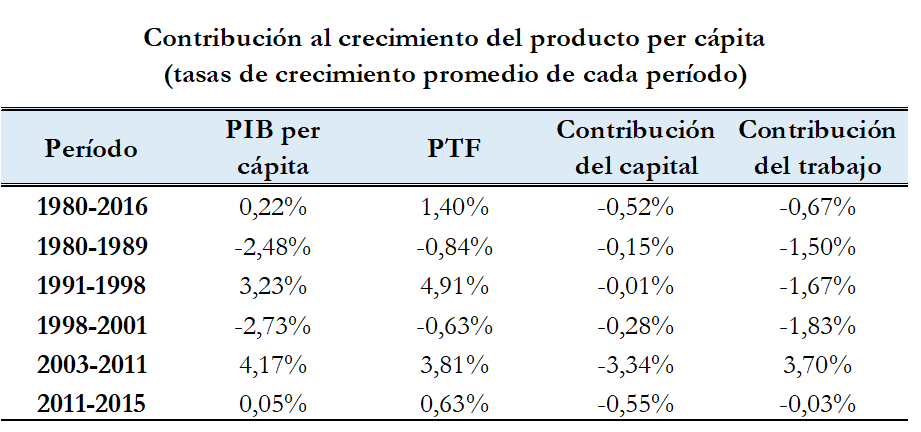
\includegraphics[scale=0.6]{../Figures/C17.4.png} 
\end{frame}
\begin{frame}{La eficiencia de mercado en términos gráficos}
  \begin{itemize}
    \item Sabemos que la pendiente negativa de la demanda refleja la disposición a pagar.
    \item Sin embargo no es lo que \textbf{efectivamete} pagan los consumidores\dots
    \item Esta diferencia entre lo que está dispuesto a pagar una persona y lo que efectivamente paga es un excedente.
    \item Este excedente lo llamaremos \textbf{excedente del consumidor}.
  \end{itemize}
  \centering
  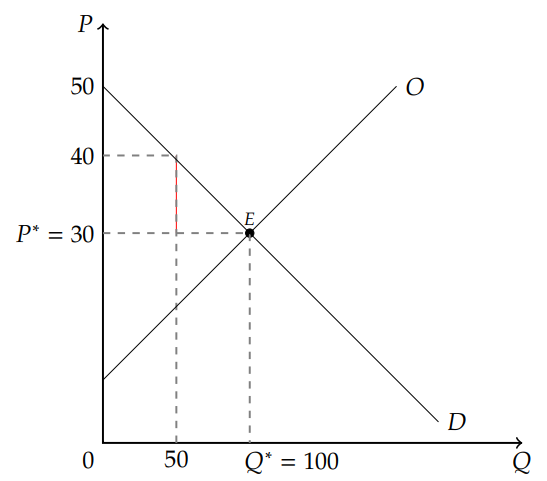
\includegraphics[scale=0.4]{../Figures/C17.5.png}
  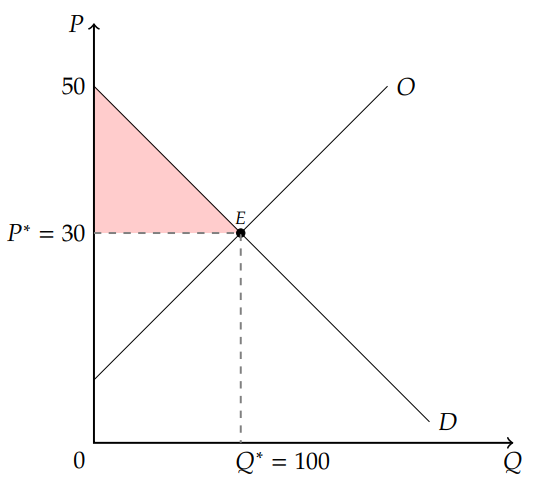
\includegraphics[scale=0.4]{../Figures/C17.6.png}
\end{frame}

\begin{frame}{La eficiencia de mercado en términos gráficos}
  \begin{itemize}
    \item Algo similar sucede por el lado de la oferta\dots
    \item Los productores que estén dispuestos a vender su producto a un precio menor al precio de equilibrio tienen una ganancia representada por la diferencia entre lo que estaban dispuestos a recibir y lo que efectivamente reciben.
    \item Este excedente lo llamaremos \textbf{excedente del productor}.
  \end{itemize}
  \centering
  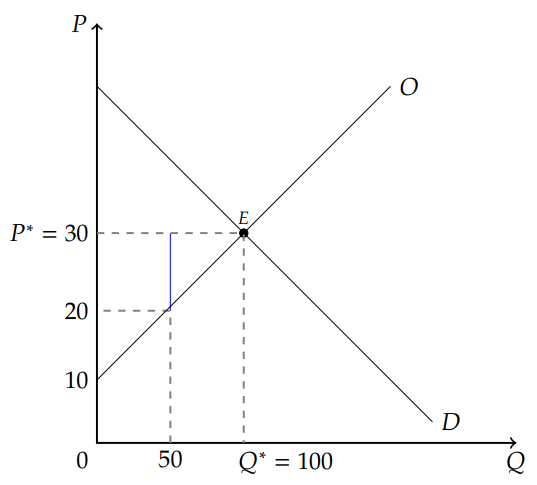
\includegraphics[scale=0.4]{../Figures/C17.7.png}
  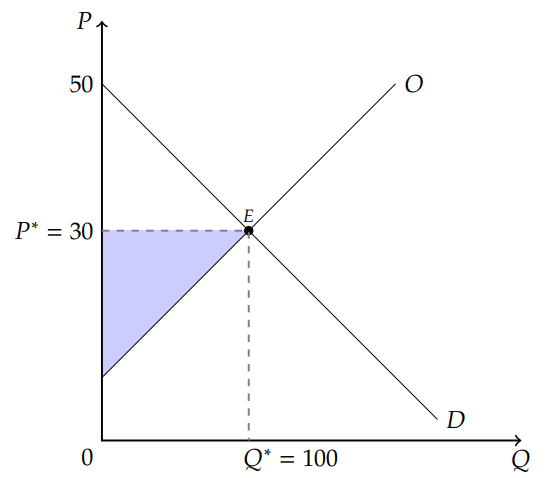
\includegraphics[scale=0.4]{../Figures/C17.8.png}
\end{frame}

\begin{frame}{La eficiencia de mercado en términos gráficos}
  \begin{itemize}
    \item A la suma del excedente del consumidor y del productor se la denomina excedente total.
    \item La eficiencia de mercado se refiere a la maximización del excedente total.
    \item Cuando la asignación no es la de equilibrio de mercado, existen ganancias o beneficios no explotados.
  \end{itemize}
  \centering
  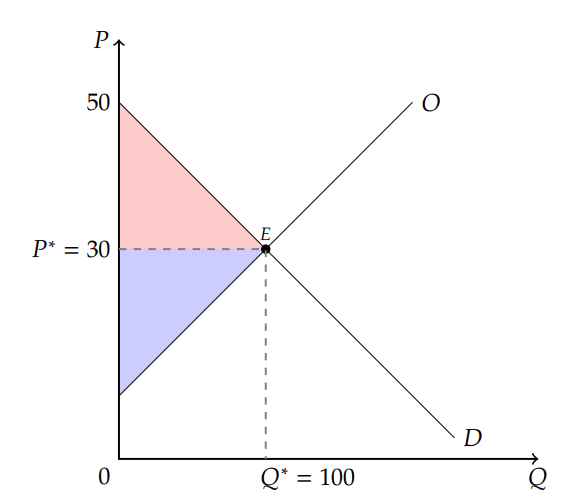
\includegraphics[scale=0.5]{../Figures/C17.9.png}
\end{frame}

\begin{frame}{La eficiencia de mercado en términos gráficos}
  \begin{boxA}
    \centering
    Llamamos perdida de peso muerto a los beneficios no explotados que se generan cuando la asignación no es un equilibrio o es un equlibrio \textit{distinto} al de competencia perfecta.
  \end{boxA}
  \centering
  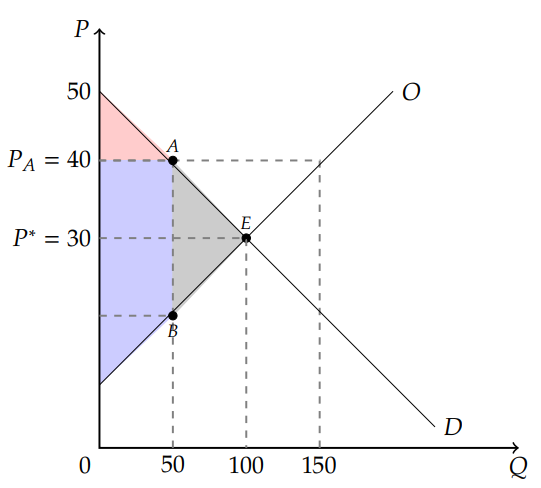
\includegraphics[scale=0.4]{../Figures/C17.10.png}
  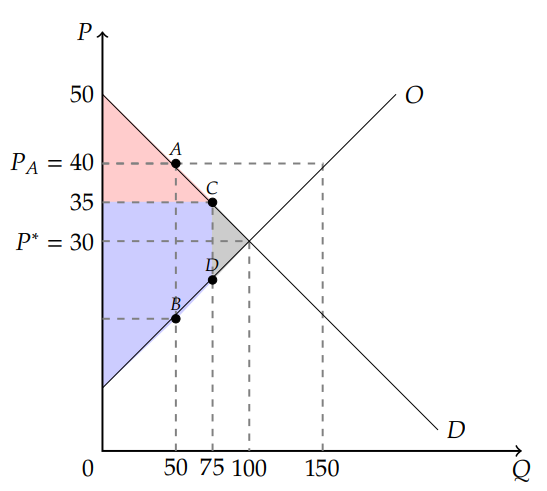
\includegraphics[scale=0.4]{../Figures/C17.11.png}
\end{frame}

\begin{frame}{Elasticidad}

  \begin{itemize}
    \item La pendiente de las curvas de oferta y demanda tiene información valiosa que no hemos discutido todavía.
    \item La reacción que tenga la cantidad demandada o ofrecida ante un cambio en alguno de los factores involucrados en el equilibrio va a variar de acuerdo a si la demanda o la oferta son más o menos empinadas.
    \item Para medir la forma en las que los consumidores y los productores responden a los cambios en los factores que determinan la demanda y la oferta, utilizaremos un nuevo concepto: el de la \textbf{elasticidad}. 
  \end{itemize}
  \begin{boxA}
    \centering
    La elasticidad es una medida de la respuesta o reacción \textit{relativa} que tienen los agentes frente a cambios de ciertas variables o determinantes económicos. Intuitivamente, nos dice cuanto reaccionan los consumidores o los productores ante un cambio en alguno de los factores.
  \end{boxA}
\end{frame}

\begin{frame}
\frametitle{Elasticidad precio de la demanda}
\begin{itemize}
    \item El concepto matemático que los economistas usamos para ver qué tan sensible es la cantidad que se demanda ante un cambio en el precio de un bien se denomina elasticidad precio de la demanda.
    \begin{equation*}
        \epsilon = \left|\frac{- \Delta \% Q}{\Delta \% P}\right| = \left|\frac{\frac{- \Delta Q}{Q}}{\frac{\Delta P}{P}}\right| = \left|-\frac{\Delta Q}{\Delta P} \frac{P}{Q}\right|
    \end{equation*}
    \item Debido a que la cantidad demandada de un bien está negativamente relacionada con el precio del bien, el cambio porcentual en la cantidad siempre tendrá un signo opuesto al del cambio porcentual en el precio.
    \item ¿Como interpretarlo? Como el cambio \% que se produce en la cantidad demandada ante un cambio de 1\% en el precio.
    \end{itemize}
\end{frame}

\begin{frame}{Elasticidad precio de la demanda}
  \begin{itemize}
    \item Si ante un cambio en el precio de un bien, la cantidad
    demandada cambia en una proporción menor al cambio proporcional
    del precio, se dice que la demanda es \textbf{inelástica}.
    \item Esto sucede siempre que la elasticidad sea \textbf{menor a 1}.
    \item En el caso en el que la elasticidad sea 0, la demanda es \textbf{perfectamente inelástica}.
  \end{itemize}
    \centering
  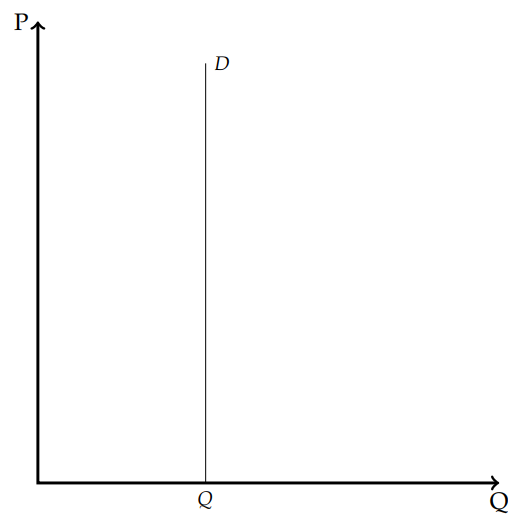
\includegraphics[scale=0.4]{../Figures/C16.1.png}
  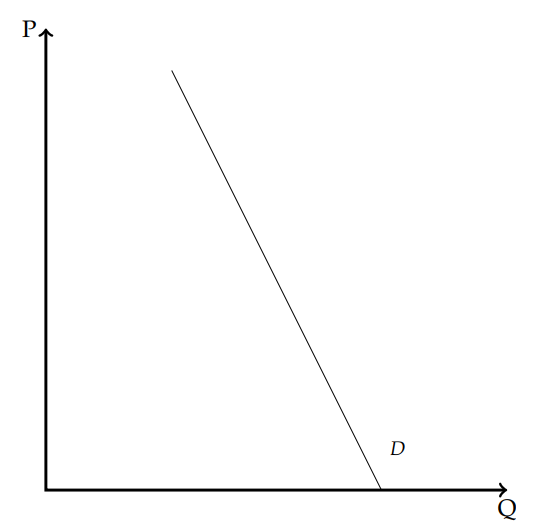
\includegraphics[scale=0.4]{../Figures/C16.2.png}
\end{frame}

\begin{frame}{Elasticidad precio de la demanda}
  \begin{itemize}
    \item Si ante un cambio en el precio de un bien, la cantidad
    demandada cambia en una proporción mayor al cambio proporcional
    del precio, se dice que la demanda es \textbf{elastica}.
    \item Esto sucede siempre que la elasticidad sea \textbf{mayor a 1}.
    \item En el caso en el que la elasticidad sea $\infty$, la demanda es \textbf{perfectamente elástica}.
  \end{itemize}
  \centering
  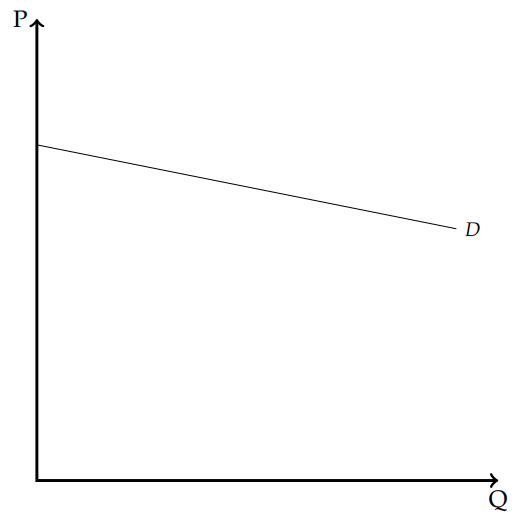
\includegraphics[scale=0.4]{../Figures/C16.3.png}
  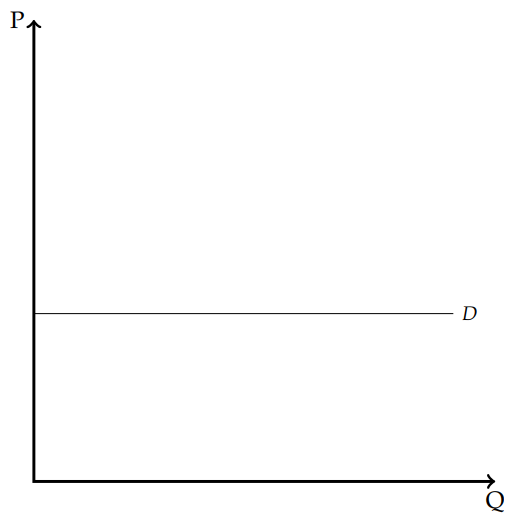
\includegraphics[scale=0.4]{../Figures/C16.5.png}
\end{frame}


\begin{frame}
\frametitle{Elasticidad precio de la demanda}
  \begin{itemize}
    \item Medida de sensibilidad: ¿Cuál es el cambio \% en la cantidad demandada ante un cambio de 1\% en el precio?
    \begin{itemize}
        \item Usamos el modulo para facilitar la interpretación! 
    \end{itemize}
    \item ¿Qué tan elástica?
    \begin{itemize}
      \item Si $\epsilon > 1$ decimos que la demanda es elástica
      \item Si $\epsilon = 1$ decimos que la demanda es unitaria
      \item Si $\epsilon < 1$ decimos que la demanda es inelástica
    \end{itemize}
  \end{itemize}
\end{frame}

\begin{frame}{Determinantes de la elasticidad precio de la demanda}
  \begin{itemize}
    \item \textbf{Disponibilidad de sustitutos cercanos}. Bienes con sustitutos cercanos tienden a tener demandas más elásticas.
    \item \textbf{La necesidad de consumo}. Cuanto más necesario sea el consumo de un bien o servicio, menor capacidad de
    respuesta tendrá el consumidor y más inelástica será la demanda.
    \item \textbf{La temporalidad de ajuste en el consumo}. Mientras más largo
    sea el período temporal que estemos considerando para el ajuste en las cantidades,
    los bienes tienden a tener demandas más elásticas, precisamente
    porque los consumidores pueden ajustar su consumo con el tiempo.
  \end{itemize}
\end{frame}

\begin{frame}{Elasticidad Puntual y Pendiente}
  \begin{footnotesize}
    \begin{equation*}
      \epsilon = \left|\frac{- \Delta \% Q}{\Delta \% P}\right| = \left|\frac{\frac{- \Delta Q}{Q}}{\frac{\Delta P}{P}}\right| = \left|-\frac{\Delta Q}{\Delta P} \frac{P}{Q}\right|\,\,\,\,\,\,\text{y}\,\,\,\,\,\, \text{pend} = \frac{\Delta P}{\Delta Q}
    \end{equation*}
    
  \end{footnotesize}
  \begin{itemize}
    \item La pendiente forma parte del concepto de elasticidad. Una demanda muy empinada es relativamente inelástica, y una bastante plana es elástica.
    \item ¡Ojo! La elasticidad puede cambiar a medida que nos movemos a lo largo de la curva de demanda, aun si la pendiente no lo hace.
  \end{itemize}
    \centering
    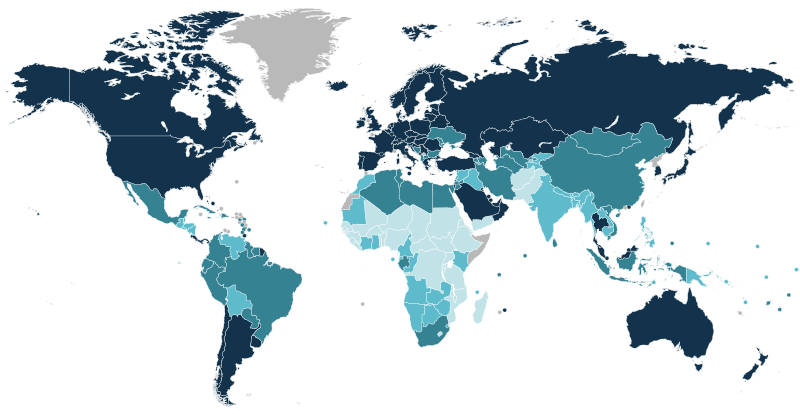
\includegraphics[scale=0.35]{../Figures/C16.7.png}
\end{frame}

\begin{frame}
    \frametitle{Elasticidad constante}
    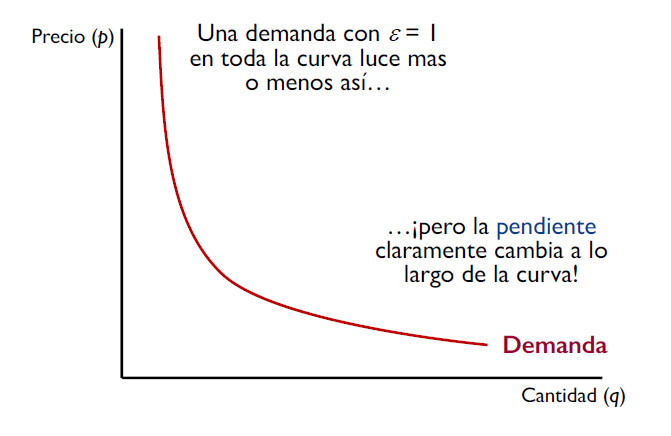
\includegraphics[scale=0.6]{../Figures/Tema_06.45_elasticidad.png}
\end{frame}

\begin{frame}
  \frametitle{Pendiente constante}
  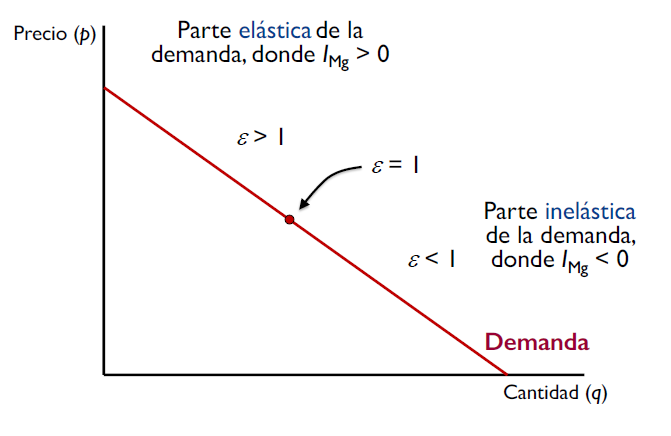
\includegraphics[scale=0.6]{../Figures/Tema_06.46_elasticidad2.png}
\end{frame}

\begin{frame}
\frametitle{Ingreso total y elasticidad}
\begin{itemize}
    \item El impacto de un cambio de precio en los ingresos totales, depende de la elasticidad de la demanda.
    \item Si la demanda es inelástica un incremento en el precio provoca un decremento en la cantidad demandada proporcionalmente más pequeño, por lo cual los ingresos totales se incrementan.
    \item En esa misma demanda, un descenso en el precio provoca un aumento en la cantidad demandada proporcionalmente más pequeño también, por lo cual los ingresos totales disminuyen.
    \item Si la curva de la demanda es elástica, un incremento en el precio provoca una disminución en la cantidad demandada proporcionalmente más grande, por lo que los ingresos totales disminuyen.
    \item En esa misma demanda, un descenso en el precio provoca un aumento en la cantidad demandada proporcionalmente más grande, por lo que los ingresos totales aumentan.
\end{itemize}
\end{frame}

\begin{frame}{Elasticidad Punto Medio}
  \begin{itemize}
      \item Hay otra forma de calcular la elasticidad, \textbf{la elasticidad punto medio}.
      \item Se utiliza para calcular la elasticidad entre dos puntos
      específicos de la curva de demanda que enfrenta una firma y se define
      de la siguiente manera:
    \end{itemize}
    \begin{equation*}
      \epsilon = \left|\frac{- \Delta \% Q}{\Delta \% P}\right|= \left|\frac{- \Delta Q}{\Delta P} \frac{\bar Q}{\bar P}\right| = \left|\frac{\frac{- \Delta Q}{\frac{(Q_2+Q_1)}{2}}}{\frac{\Delta P}{\frac{(P_2+P_1)}{2}}}\right| = \left|-\frac{\Delta Q}{\Delta P} \frac{\frac{(P_2+P_1)}{2}}{\frac{(Q_2+Q_1)}{2}}\right|
    \end{equation*}
\end{frame}


\begin{frame}
\frametitle{Elasticidad precio de la oferta}
    \begin{equation*}
      \epsilon^{O}_p = \frac{\Delta \% Q}{\Delta \% P} = \frac{\frac{\Delta Q}{Q}}{\frac{\Delta P}{P}} = \frac{\Delta Q}{\Delta P} \frac{P}{Q}
    \end{equation*}
    \begin{itemize}
      \item \textbf{Elástica}: Un cambio en el precio del bien provoca un cambio
      proporcional mayor en la oferta del bien.
      \item \textbf{Inelástica}: Un cambio en el precio de un bien, su
      cantidad ofertada cambia en una proporción menor al cambio en
      el precio.
      \item \textbf{Unitaria}: un cambio en el precio se traduce como un cambio en la
      cantidad ofertada en la misma proporción.
      \item \textbf{Perfectamente elástica} y \textbf{Perfectamente inelástica}.
      \item \textbf{Factores}: Posibilidad de stockearse, tiempo de producción, procesos productivos, etc.    
    \end{itemize}
\end{frame}

\begin{frame}{Elasticidad Cruzada}
  \begin{itemize}
    \item Elasticidad Cruzada: Es el cambio porcentual en las cantidades demandadas cuando el precio de otro bien cambia 1\%.
    \begin{equation*}
      \epsilon_{x,y} = \frac{\Delta \% Q_x}{\Delta \% P_y}
    \end{equation*}
    \begin{itemize}
        \item Si la elasticidad cruzada es 0, no hay relación entre ambos bienes.
        \item Si esta elasticidad es mayor a 0, los bienes son sustitutos, es decir, cuando se incrementa el precio de y aumenta la cantidad demandada de x; 
        \item Si es menor a 0, los bienes son complementarios, es decir, si aumenta el precio de y baja la cantidad demandada de x.
    \end{itemize}
  \end{itemize}
\end{frame}

\begin{frame}{Elasticidad Ingreso}
  \begin{itemize}
    \item Elasticidad Ingreso: Es el cambio porcentual en las cantidades demandadas cuando el ingreso cambia 1\%.
    \begin{equation*}
      \epsilon_I = \frac{\Delta \% Q}{\Delta \% I}
    \end{equation*}    
    \begin{itemize}
        \item Si se mueven en conjunto ingreso y cantidades, la elasticidad ingreso será mayor a 0 y estamos en presencia de bienes normales.
        \item si la elasticidad ingreso es negativa, ante un cambio en el ingreso la cantidad demandada del bien se mueve en la dirección opuesta. En este caso estamos en presencia de un bien inferior.
        \item A su vez, si la elasticidad ingreso es mayor a 1 decimos que estamos ante un bien de lujo.
    \end{itemize}
    \item En estos ultimos casos, no usamos modulo. En la oferta no lo hicimos porque la pendiente es positiva y, por ende, la elasticidad siempre lo será también.
    \item En los otros dos casos, conocer el signo nos ayuda a interpretar que tipo de bienes son, por lo que es necesario sacar el modulo para interpretar completamente.
\end{itemize}
\end{frame}

\end{document}